

As the distribution coefficient $K_d$, and therefore the retardation
coefficient $R_f$ increase, contaminants tend toward the solid phase. An
increase in these coefficients, then, has the effect of limiting dissolved
concentration.

In the parametric sensitivity analysis reported in \cite{huff_key_2012},
the expected inverse relationship between the retardation factor and resulting
peak annual dose was found for all elements that were not assumed to be
effectively infinitely soluble.  In the low retardation coefficient cases, a
regime is established in which the peak annual dose is entirely unaffected by
changes in retardation coefficient.

For large values of retardation coefficient, the sensitivity to small changes
in the retardation coefficient increases dramatically. In that sensitive
regime, the change in peak annual dose is inversely related to the retardation
coefficient. Between these two regimes was a transition regime, in which the
$K_d$ factor ranges from $1\times10^{-5}$ to $5\times10^{0} [-]$.

It is clear from Figure \ref{fig:KdSumFactor} that
for retardation coefficients greater than a threshold, the
relationship between peak annual dose and retardation coefficient is a strong
inverse one.

\begin{figure}[ht]
\centering
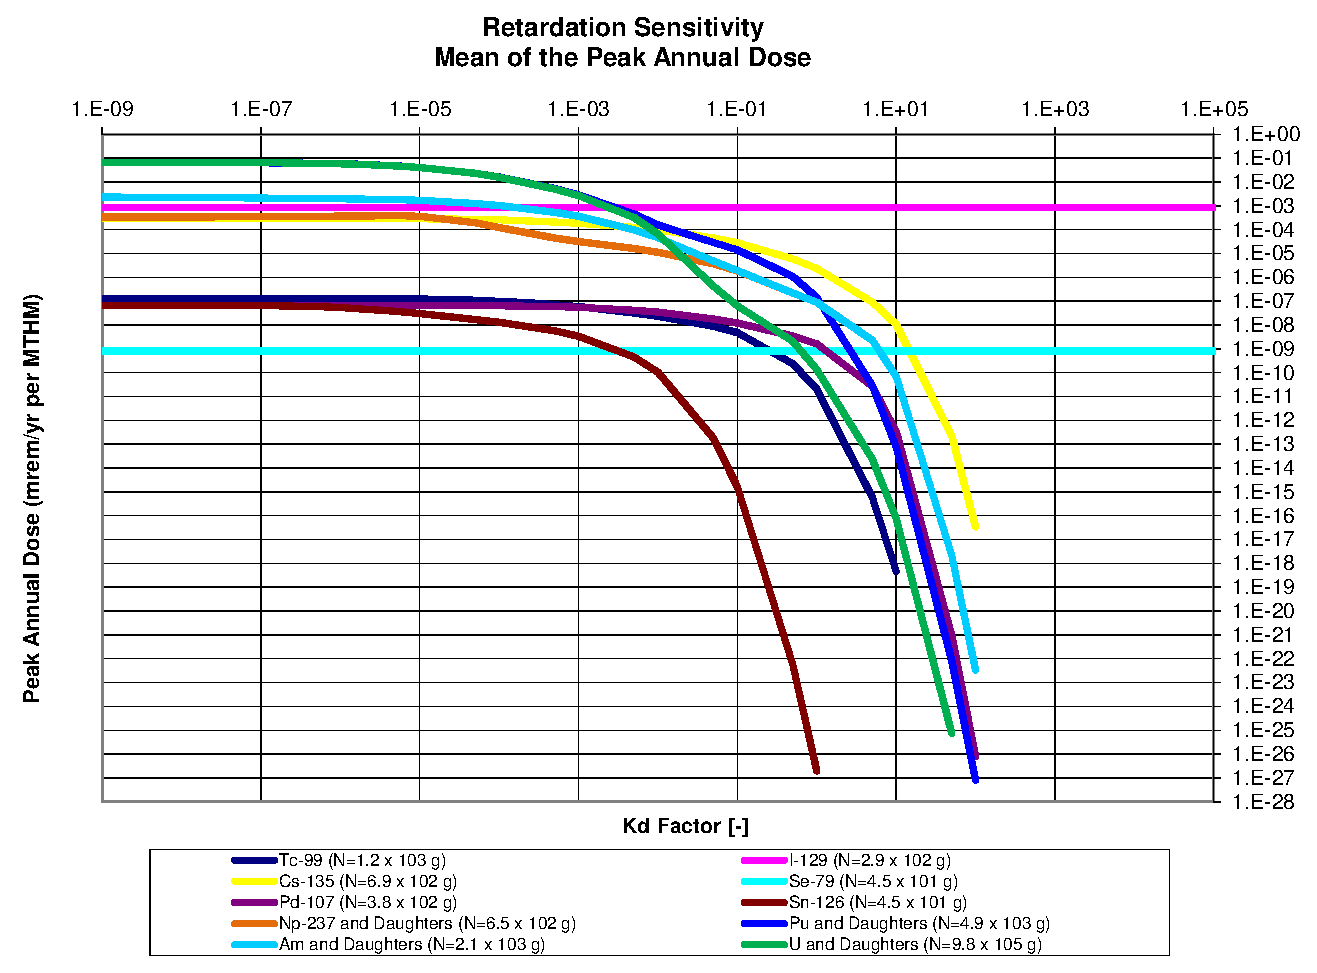
\includegraphics[width=0.7\linewidth]{./results/images/Retardation_Summary_kdFactor.eps}
\caption[$K_d$ factor sensitivity in Clay GDSM]{$K_d$ factor sensitivity in 
        DOE Clay GDSM, reproduced from \cite{huff_key_2012}.
The peak annual dose due to an inventory,
$N$, of each isotope.}
\label{fig:KdSumFactor}
\end{figure}

\FloatBarrier
